%%%%%%%%%%%%%%%%%%%%%%%%%%%%%%%%%%%%%%%%%
% Beamer Presentation
% LaTeX Template
% Version 1.0 (10/11/12)
%
% This template has been downloaded from:
% http://www.LaTeXTemplates.com
%
% License:
% CC BY-NC-SA 3.0 (http://creativecommons.org/licenses/by-nc-sa/3.0/)
%
%%%%%%%%%%%%%%%%%%%%%%%%%%%%%%%%%%%%%%%%%

%----------------------------------------------------------------------------------------
%	PACKAGES AND THEMES
%----------------------------------------------------------------------------------------

\documentclass{beamer}

\mode<presentation> {

% The Beamer class comes with a number of default slide themes
% which change the colors and layouts of slides. Below this is a list
% of all the themes, uncomment each in turn to see what they look like.

%\usetheme{default}
%\usetheme{AnnArbor}
%\usetheme{Antibes}
%\usetheme{Bergen}
%\usetheme{Berkeley}
\usetheme{Berlin}
%\usetheme{Boadilla}
%\usetheme{CambridgeUS}
%\usetheme{Copenhagen}
%\usetheme{Darmstadt}
%\usetheme{Dresden}
%\usetheme{Frankfurt}
%\usetheme{Goettingen}
%\usetheme{Hannover}
%\usetheme{Ilmenau}
%\usetheme{JuanLesPins}
%\usetheme{Luebeck}
%\usetheme{Madrid}
%\usetheme{Malmoe}
%\usetheme{Marburg}
%\usetheme{Montpellier}
%\usetheme{PaloAlto}
%\usetheme{Pittsburgh}
%\usetheme{Rochester}
%\usetheme{Singapore}
%\usetheme{Szeged}
%\usetheme{Warsaw}

% As well as themes, the Beamer class has a number of color themes
% for any slide theme. Uncomment each of these in turn to see how it
% changes the colors of your current slide theme.

%\usecolortheme{albatross}
\usecolortheme{beaver}
%\usecolortheme{beetle}
%\usecolortheme{crane}
%\usecolortheme{dolphin}
%\usecolortheme{dove}
%\usecolortheme{fly}
%\usecolortheme{lily}
%\usecolortheme{orchid}
%\usecolortheme{rose}
%\usecolortheme{seagull}
%\usecolortheme{seahorse}
%\usecolortheme{whale}
%\usecolortheme{wolverine}

%\setbeamertemplate{footline} % To remove the footer line in all slides uncomment this line
%\setbeamertemplate{footline}[page number] % To replace the footer line in all slides with a simple slide count uncomment this line

%\setbeamertemplate{navigation symbols}{} % To remove the navigation symbols from the bottom of all slides uncomment this line
}

\usepackage{graphicx} % Allows including images
\usepackage{booktabs} % Allows the use of \toprule, \midrule and \bottomrule in tables
\usepackage{graphicx, subcaption}
\usepackage{amssymb, mathtools}
\usepackage{algorithm, algpseudocode}

%
\DeclarePairedDelimiter{\inner}{\langle}{\rangle}

% 
\usepackage{adjustbox}
\usepackage{tikz}
\usetikzlibrary{positioning,shapes.geometric, arrows, fit,calc}
\tikzstyle{block} = [draw, rectangle, fill=orange!50, text width=8em, text centered, minimum height=15mm, node distance=10em]
\tikzstyle{container} = [draw, rectangle, dashed, inner sep=0.7em]
\tikzstyle{arrow} = [thick,->,>=stealth]

%macros from Bob Gray
\usepackage{"./macro/GrandMacros"}
\usepackage{"./macro/Macro_BIO235"}

\usepackage[normalem]{ulem}
\makeatletter
\let\@@magyar@captionfix\relax
\makeatother
%----------------------------------------------------------------------------------------
%	TITLE PAGE
%----------------------------------------------------------------------------------------


\begin{document}

\title{Robust Test for Nonlinear Interaction \\ using \\ 
Cross-Validated Kernel Ensemble}
\author{\textbf{Wenying Deng, Jeremiah Zhe Liu}\\ 
Department of Biostatistics \\
Harvard University}
\date{Biostat Seminar \\ \today}
\begin{frame}
\titlepage
\end{frame}

\begin{frame}
\frametitle{Contents} % Table of contents slide, comment this block out to remove it
\tableofcontents[hideallsubsections]
% Throughout your presentation, if you choose to use \section{} and \subsection{} commands, these will automatically be printed on this slide as an overview of your presentation
\end{frame}

%----------------------------------------------------------------------------------------
%	PRESENTATION SLIDES
%----------------------------------------------------------------------------------------
\section{Problem Setup} 

\begin{frame}
\frametitle{Background}

Consider a nutrition-environment interaction study for continuous infant health outcome $y_i$. For observation i, we have:
\begin{enumerate}
\item $\mu$: the fixed effect of background covariates, assuming the same across all observations.
\item $\bx_{1,i}$: 2 $\sim$ 10 nutrients variables (e.g. Vitamin, Folate,  etc)
\item $\bx_{2,i}$: 2 $\sim$ 10 environmental exposure (e.g. $PM_{2.5}$, pesticides, etc)
\end{enumerate}

Effect of $\bx_{1,i}$ and $\bx_{2,i}$ on $y_i$ is {\color{red}nonlinear}. \\ 
$ $ \\

We observe $n \approx 100$ such records, and want to investigate whether mother's nutrients intake during pregnancy $\bx_1$ modifies the effects of prenatal exposures to $\bx_2$, i.e. {\color{red}nonlinear interaction} between $\bx_1$ and $\bx_2$.

\end{frame}

\begin{frame}
\frametitle{Problem Setup}
\begin{itemize}[<+->]
\item True Model
$$y_i = \mu + h(\bx_{1i}, \bx_{2i}) + \epsilon_i, \quad \epsilon_i \sim N(0, \sigma^2)$$
where
$$h(\bx_{1i}, \bx_{2i}) = \Big[ 
h_1(\bx_{1i}) + h_2(\bx_{2i})  \Big] + h_{12}(\bx_{1i}, \bx_{2i})$$
\begin{itemize}
\item $h_{1} \in \Hsc_1$ and $h_2 \in \Hsc_2$ are the \textbf{main effect function}s
\item $h_{12}(\bx_{1i}, \bx_{2i}) \in \Hsc_{12}$ is the \textbf{pure interaction function}
\begin{itemize}
\item $h_{12} \perp h_1$ and  $h_{12} \perp h_2$.
\end{itemize}
\item $\Hsc_1$, $\Hsc_2$ and $\Hsc_{12}$ are \textbf{UNKNOWN}.
\end{itemize}
\end{itemize}
\end{frame}

\begin{frame}

\frametitle{Hypothesis}
\begin{itemize}
\item Model 
$$y_i = \mu + h(\bx_{1i}, \bx_{2i}) + \epsilon_i$$
where
$$h(\bx_{1i}, \bx_{2i}) = \Big[ 
h_1(\bx_{1i}) + h_2(\bx_{2i})  \Big] + h_{12}(\bx_{1i}, \bx_{2i})$$
\item Hypothesis 
\begin{align*}
&H_0: h \in \Hsc_0 = \Hsc_1 \oplus \Hsc_2 \\
&H_a: h \in \Hsc_a = \Hsc_1 \oplus \Hsc_2 \oplus \Hsc_{12}
\end{align*}
\end{itemize}
\end{frame}


\begin{frame}
\frametitle{Overview}
\begin{itemize}
\item \textbf{Assumption}:
Given a library of kernels $\{k_d(\bx, \bx')\}_{d=1}^D$, assume 
$$h_0(\bx) = \sum_{d=1}^D u_d h_d(\bx), \qquad \sum_{d=1}^D u_d = 1, u_d > 0$$
where $h_d \in \Hsc_d$, the function space corresponds to $k_d(\bx, \bx')$.

\end{itemize}
\end{frame}

\begin{frame}
\frametitle{Overview}
\begin{itemize}
\item \textbf{Model}: 
\begin{align*}
\by 
&= \bmu + h_0(\bx) \\
&= \bmu + \sum_{d=1}^D u_d h_d(\bx) \\
&= \bmu + \sum_{d=1}^D u_d \bK_d \balpha_d
\end{align*}
\end{itemize}
\end{frame}

\begin{frame}
\frametitle{Overview}
\begin{adjustbox}{max totalsize={1\textwidth}{.7\textheight}, center}
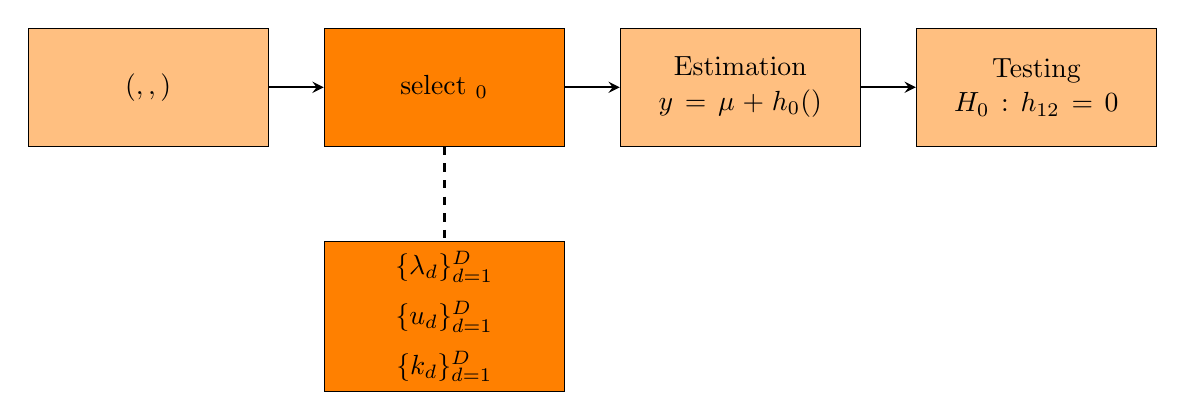
\begin{tikzpicture}[auto]
\linespread{1}
\node [block, fill=orange] (fix) {select $\Hsc_0$};
\node [block, left = 0.7cm of fix] (data) {$(\by, \bmu, \bX)$};
\node [block, below = 1.2cm of fix, fill=orange] (dd) {$\{\lambda_d\}_{d=1}^D$\\ \vspace{.6em}$\{u_d\}_{d=1}^D$\\ \vspace{.6em}$\{k_d\}_{d=1}^D$};
\node [block, right = 0.7cm of fix] (REML) 
{Estimation \\[0.05em] $y = \mu + h_0(\bX)$};
\node [block, right = 0.7cm of REML] (VCT) 
{Testing \\[0.05em] $H_0: h_{12} = 0$};
\draw [arrow] (data) -- (fix);
\draw [arrow] (fix) -- (REML);
\draw [arrow] (REML) -- (VCT);
\draw [dashed, very thick] (fix) -- (dd);
\end{tikzpicture}
\end{adjustbox}
\end{frame}


\begin{frame}
\frametitle{Overview}
\label{kmr}
\begin{adjustbox}{max totalsize={1\textwidth}{.7\textheight}, center}
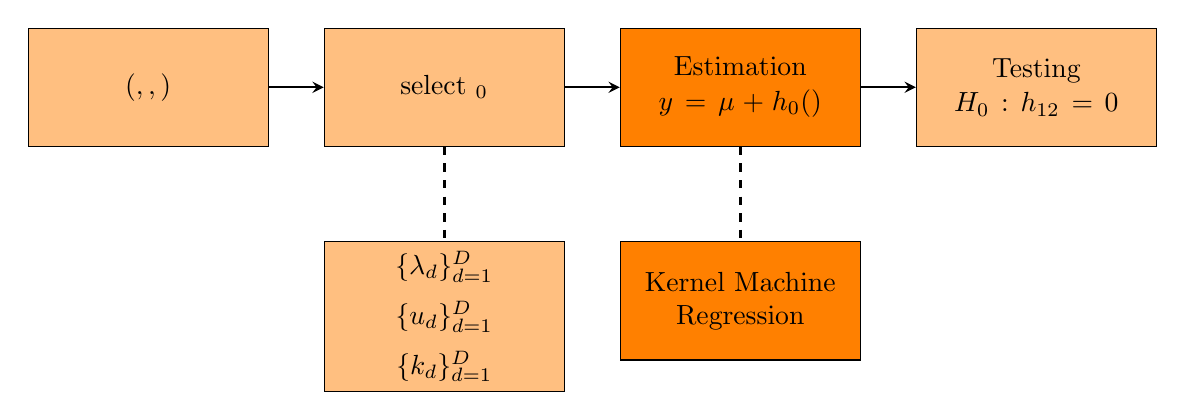
\begin{tikzpicture}[auto]
\linespread{1}
\node [block] (fix) {select $\Hsc_0$};
\node [block, left = 0.7cm of fix] (data) {$(\by, \bmu, \bX)$};
\node [block, below = 1.2cm of fix] (dd) {$\{\lambda_d\}_{d=1}^D$\\ \vspace{.6em}$\{u_d\}_{d=1}^D$\\ \vspace{.6em}$\{k_d\}_{d=1}^D$};
\node [block, right = 0.7cm of fix, fill=orange] (REML) 
{Estimation \\[0.05em] $y = \mu + h_0(\bX)$};
\node [block, right = 0.7cm of REML] (VCT) 
{Testing \\[0.05em] $H_0: h_{12} = 0$};
\node [block, below = 1.2cm of REML, fill=orange] (ss) {Kernel Machine Regression};
\draw [arrow] (data) -- (fix);
\draw [arrow] (fix) -- (REML);
\draw [arrow] (REML) -- (VCT);
\draw [dashed, very thick] (fix) -- (dd);
\draw [dashed, very thick] (REML) -- (ss);
\end{tikzpicture}
\end{adjustbox}
\hyperlink{est}{\beamergotobutton{Estimates}}
\end{frame}


\begin{frame}
\frametitle{Overview}
\begin{adjustbox}{max totalsize={1\textwidth}{.7\textheight}, center}
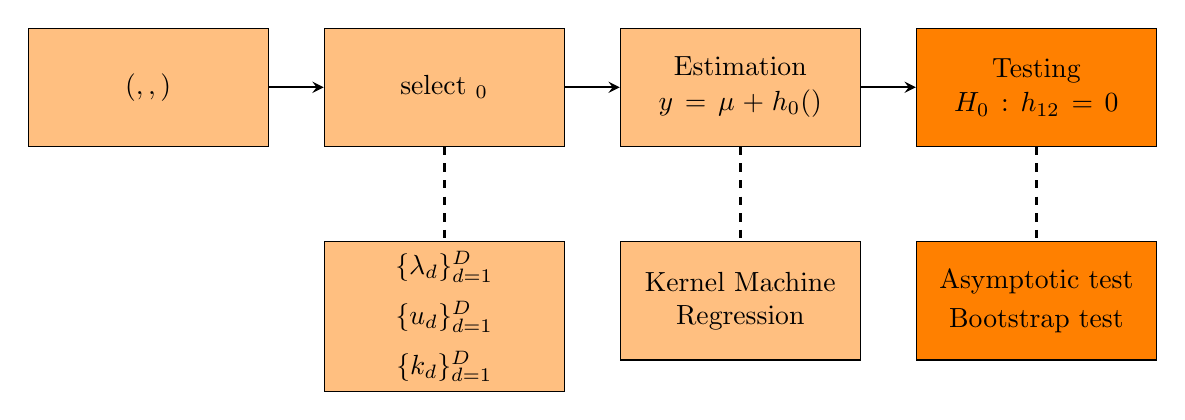
\begin{tikzpicture}[auto]
\linespread{1}
\node [block] (fix) {select $\Hsc_0$};
\node [block, left = 0.7cm of fix] (data) {$(\by, \bmu, \bX)$};
\node [block, below = 1.2cm of fix] (dd) {$\{\lambda_d\}_{d=1}^D$\\ \vspace{.6em}$\{u_d\}_{d=1}^D$\\ \vspace{.6em}$\{k_d\}_{d=1}^D$};
\node [block, right = 0.7cm of fix] (REML) 
{Estimation \\[0.05em] $y = \mu + h_0(\bX)$};
\node [block, right = 0.7cm of REML, fill=orange] (VCT) 
{Testing \\[0.05em] $H_0: h_{12} = 0$};
\node [block, below = 1.2cm of REML] (ss) {Kernel Machine Regression};
\node [block, below = 1.2cm of VCT, fill=orange] (hh) {Asymptotic test\\ \vspace{.2em}Bootstrap test};
\draw [arrow] (data) -- (fix);
\draw [arrow] (fix) -- (REML);
\draw [arrow] (REML) -- (VCT);
\draw [dashed, very thick] (fix) -- (dd);
\draw [dashed, very thick] (REML) -- (ss);
\draw [dashed, very thick] (VCT) -- (hh);
\end{tikzpicture}
\end{adjustbox}
\end{frame}


%------------------------------------------------
\section{Cross-Validated Ensemble of Kernels} 
%------------------------------------------------

\begin{frame}<beamer>
\tableofcontents[currentsection]
\end{frame}


\subsection{Tuning Parameter Selection}
\begin{frame}
Denote 
$$\bA_\lambda=\bK(\bX, \bX)[\bK(\bX, \bX)+\lambda \bI]^{-1}$$
and
$$\by^\star=\by-\hat{\bmu}, \quad \hat{\mu}=\frac{1}{n}\sum_{i=1}^ny_i$$
\begin{itemize}
\item $tr(\bA_\lambda)$ is the effective number of model parameters
\item $\by^\star$ is centered
\end{itemize}
\end{frame}


\begin{frame}
\begin{itemize}
\item LooCV: leave-one-out Cross Validation
$$\underset{\lambda \in \Lambda}{argmin}\;\Big\{log\;\by^{\star T}[\bI-diag(\bA_\lambda)-\frac{1}{n}\bI]^{-1}(\bI-\bA_\lambda)^2[\bI-diag(\bA_\lambda)-\frac{1}{n}\bI]^{-1}\by^\star \Big\}$$
\item AICc: small sample size version of AIC
$$\underset{\lambda \in \Lambda}{argmin}\Big\{log\; \by^{\star T}(\bI-\bA_\lambda)^2\by^\star+\frac{2[tr(\bA_\lambda)+2]}{n-tr(\bA_\lambda)-3}\Big\}$$
\item GCVc: small sample size version of GCV
$$\underset{\lambda \in \Lambda}{argmin}\Big\{log\; \by^{\star T}(\bI-\bA_\lambda)^2\by^\star-2log[1-\frac{tr(\bA_\lambda)}{n}-\frac{2}{n}]_+\Big\}$$
\item GMPML: Generalized Maximum Profile Marginal Likelihood
$$\underset{\lambda \in \Lambda}{argmin}\Big\{log\; \by^{\star T}(\bI-\bA_\lambda)\by^\star-\frac{1}{n-1}log \mid \bI-\bA_\lambda \mid \Big\}$$
\end{itemize}
\end{frame}

\begin{frame}
\label{lambda: aic_gcv}
Note: $\lambda_{AIC}$ is always smaller than $\lambda_{GCV}$. \hyperlink{proof: aic_gcv}{\beamergotobutton{Derive}}
\end{frame}


\subsection{Ensemble Strategy}
\begin{frame}
\begin{itemize}
\item ERM: Empirical Risk Minimization
$$\hat{\bu}=\underset{\bu \in \Delta}{argmin}\parallel \sum_{d=1}^Du_d\hat{\bepsilon}_d\parallel^2 \quad where\; \Delta=\{\bu \mid \bu \geq 0, \parallel \bu \parallel_1=1\}$$
\item AVE: Simple Averaging
$$u_d=1/D \quad \mbox{for} \quad d=1,2,...D$$
\item EXP: Exponential Weighting
$$u_d(\beta)=\frac{exp(-\parallel \hat{\bepsilon}_d \parallel_2^2/\beta)}{\sum_{d=1}^Dexp(-\parallel \hat{\bepsilon}_d \parallel_2^2/\beta)}\quad \mbox{for} \quad d=1,2,...D$$
\end{itemize}
\end{frame}


\begin{frame}
Then produce the final ensemble prediction:
\begin{align*}
\hat{\bh}_0=\sum_{d=1}^D \hat{u}_d \bh_d=\sum_{d=1}^D \hat{u}_d \bA_{d,\hat{\lambda}_d}\by^\star=\hat{\bA}\by^\star
\end{align*}
where $\hat{\bA}=\sum_{d=1}^D \hat{u}_d \bA_{d,\hat{\lambda}_d}$ is the ensemble matrix.
\end{frame}


\subsection{Kernel Choice}
\begin{frame}
\begin{itemize}
\item Polynomial Kernel: polynomial functions $$k(\bx, \bx') = (b + \bx^T\bx')^p$$
\item Gaussian Kernel: infinitely differentiable functions
$$k(\bx, \bx') =exp\Big(-\frac{\mid\bx-\bx'\mid^2}{2l^2}\Big)$$
\item Mat\'{e}rn 1/2 Kernel:  continuous, non-differentiable functions $$k(\bx, \bx') = exp(-\frac{\mid\bx-\bx'\mid}{l})$$
\item Mat\'{e}rn 5/2 Kernel:  twice-differentiable functions
$$k(\bx, \bx') = (1 + \frac{\sqrt{5}\mid\bx-\bx'\mid}{l} +\frac{5\mid\bx-\bx'\mid^2}{3l^2}) exp(-\frac{\sqrt{5}\mid\bx-\bx'\mid}{l})$$
\end{itemize}
\end{frame}


\section{Hypothesis Test}

\begin{frame}<beamer>
\tableofcontents[currentsection]
\end{frame}

\subsection{Asymptotic Test}
\begin{frame}
\frametitle{Variance Component Test for Interaction}
\label{vct}
\textbf{Translate Hypothesis:}
Under LMM representation:
\begin{align*}
\by = \bmu + \bh + \bepsilon 
\qquad \mbox{where} \qquad
\bh \sim N(\bzero, \tau \bK) \qquad 
\bepsilon \sim N(\bzero, \sigma^2 \bI)
\end{align*} 
\begin{itemize}[<+->]
\item Under $H_0$: $\Hsc = \Hsc_1 \oplus \Hsc_2$,  same as \\
$k = k_1 + k_2 \quad (\Rightarrow) \quad 
\bK = \bK_1 + \bK_2$
\item Under $H_a$: $\Hsc = \Hsc_1 \oplus \Hsc_2 \oplus \Hsc_{12}$,  same as\\
$k = k_1 + k_2 + k_{12} \quad (\Rightarrow) \quad 
\bK = \bK_1 + \bK_2 + \bK_{12}$
\item So write $\bK = \bK_1 + \bK_2 + \delta *\bK_{12}$
\item Test for $H_0: \delta = 0$ using VCT  \hyperlink{vct_detail}{\beamergotobutton{Detail}}
\end{itemize}
\end{frame}


\subsection{Bootstrap Test}
\begin{frame}
\frametitle{What if our sample size is pretty small?}
\begin{center}
How to make full use of our limited sample?
\end{center}
\end{frame}

\begin{frame}
\frametitle{What if our sample size is pretty small?}
\begin{center}
\textbf{Bootstrap!}
\end{center}
\end{frame}

\begin{frame}
\frametitle{What if our sample size is pretty small?}
A good approximation to the distribution of the test statistic under sampling from the true null-hypothesis model is the distribution of the test statistic under sampling from the fitted null-hypothesis model.
\end{frame}


\begin{frame}
\begin{enumerate}[<+->]
\item Obtain parameter estimates from the original data by fitting a null-hypothesis model $$E(\by^\star)=\bK_0(\bK_0+\lambda \bI)^{-1}\by=\bA_0\by$$
\item Sample $\bY^\star$ for each individuals with a random noise, whose variance is also estimated.
\item Compute the test statistic, based on fitting the alternative-hypothesis model to the samples obtained in Step 2.
\item Repeat Steps 2 and 3 for $B$ times, to obtain an approximate distribution of the test statistic.
\item Compute the test statistic for the original data, based on fitting the alternative- hypothesis model.
\item Compute the p-value, by comparing the test statistic in Step 5 to the distribution in Step 4.
\end{enumerate}
\end{frame}


\section{Simulation Study}

\begin{frame}<beamer>
\tableofcontents[currentsection]
\end{frame}

\subsection{Data-generation Mechanism}
\begin{frame}
Generate data under
$$y=\mu+h_1(\bx_1)+h_2(\bx_2)+\delta * h_1(\bx_1) * h_2(\bx_2)+\epsilon$$
\begin{itemize}
\item Vary $\delta \in \{0, 0.1, 0.2, 0.3\}$;
\item 3 polynomial kernels ($p=1, 2, 3$) representing finite-dimensional, parametric functions of different degree of nonlinearity;
\item 3 Gaussian RBF kernels ($l=0.5, 1, 1.5$) representing smooth functions of different frequency;
\item 6 Matern kernels, with $l \in \{0.5, 1, 1.5\}$ and $\nu \in \{\frac{3}{2}, \frac{5}{2}\}$, representing functions with different frequency and differentiability.
\end{itemize}
\end{frame}


\subsection{Model Strategy}
\begin{frame}
%\label{model}
Fit null model:
$$y=\mu + h_1(\bx_1) + h_2(\bx_2)$$
using below kernels:
\begin{enumerate}
\item 3 polynomial kernels with degree ($p=1, 2, 3$); \hyperlink{poly}{\beamergotobutton{Fig1}}
\item 3 RBF kernels with wavelength ($l=0.6, 1, 2$); \hyperlink{rbf}{\beamergotobutton{Fig2}}
\item 3 polynomial kernels ($p=1, 2, 3$) and 3 RBF kernels ($l=0.6, 1, 2$); \hyperlink{poly_rbf}{\beamergotobutton{Fig3}}
\item 3 $l=1$ Matern kernels ($\nu=1/2, 3/2, 5/2$) and 3 RBF kernels ($l=0.6, 1, 2$). \hyperlink{mat_rbf}{\beamergotobutton{Fig4}}
\end{enumerate}
\end{frame}


\subsection{Result}
\begin{frame}
\label{poly}
\begin{figure}
\centering
\includegraphics[width=\linewidth]{"./plot/poly"}
\end{figure}
%\hyperlink{model}{\beamergotobutton{Model}}
\end{frame}


\begin{frame}
\label{rbf}
\begin{figure}
\centering
\includegraphics[width=\linewidth]{"./plot/rbf"}
\end{figure}
%\hyperlink{model}{\beamergotobutton{Model}}
\end{frame}


\begin{frame}
\label{poly_rbf}
\begin{figure}
\centering
\includegraphics[width=\linewidth]{"./plot/poly_rbf"}
\end{figure}
%\hyperlink{model}{\beamergotobutton{Model}}
\end{frame}


\begin{frame}
\label{mat_rbf}
\begin{figure}
\centering
\includegraphics[width=\linewidth]{"./plot/mat_rbf"}
\end{figure}
%\hyperlink{model}{\beamergotobutton{Model}}
\end{frame}

\begin{frame}
\frametitle{Main Message: Tuning Parameter Selection}
In general, 
\begin{itemize}
\item LooCV, guarantees correct Type I error, but potentially leads to low power; \hyperlink{mat_rbf}{\beamergotobutton{Fig4}}
\item AICc, powerful if base kernels are as or more complex than the true one; \hyperlink{mat_rbf}{\beamergotobutton{Fig4}}
\item GMPML, powerful if base kernels are smoother than the true one. \hyperlink{poly}{\beamergotobutton{Fig1}}
\end{itemize}
\end{frame}


\begin{frame}
\frametitle{Main Message: Ensemble Strategy}
\begin{itemize}
\item AVE is better if base kernels are simple and finite-dimensional; \hyperlink{poly}{\beamergotobutton{Fig1}}
\item ERM is better if base kernels are flexible and infinite-dimensional; \hyperlink{rbf}{\beamergotobutton{Fig2}} \hyperlink{mat_rbf}{\beamergotobutton{Fig4}}
\item In the more complex scenario... \hyperlink{poly_rbf}{\beamergotobutton{Fig3}}
\item EXP, fairly greater power except when the true kernel is strictly simpler than base kernels. \hyperlink{rbf}{\beamergotobutton{Fig2}}
\end{itemize}
\end{frame}


\begin{frame}
\begin{center}
Questions?
\end{center}
\end{frame}


\section{Appendix}

\begin{frame}
\label{est}
\frametitle{KMR as a Linear Mixed Model}
\begin{itemize}
\item KMR Estimates:
\begin{align*}
\hat{\mu} &= (\bf{1}^T (\bK_0 + \lambda * \bI)^{-1} \bf{1} )^{-1} 
\bf{1}^T (\bK_0 + \lambda * \bI)^{-1} \\
\hat{\balpha} &= (\bK_0 + \lambda * \bI)^{-1} (\by - \bf{1}* \hat{\mu})\\
\hat{\bh}_0 &= \bK_0\hat{\balpha} = 
\bK_0(\bK_0 + \lambda * \bI)^{-1} (\by - \bf{1}* \hat{\mu})
\end{align*}
\item Same solution as a LMM with random intercept $\bh$:
\begin{align*}
\by = \bmu + \bh + \bepsilon 
\qquad \mbox{where} \qquad
\bh \sim N(\bzero, \tau \bK) \qquad 
\bepsilon \sim N(\bzero, \sigma^2 \bI)
\end{align*} 
where $\sigma^2 / \tau = \lambda$
\item Estimate variance component parameters $(\tau, \sigma^2)$ using REML \hyperlink{kmr}{\beamergotobutton{Back}}
\end{itemize}
\end{frame}


\begin{frame}
\label{proof: aic_gcv}
If we denote $\bU_K$ and $\{\eta_{K, j}\}_{j=1}^n$ as the eigenvector and eigenvalues of $\bK$, then $\bA_\lambda$ adopts the form:
$$\bA_\lambda=\bU_K diag(\frac{\eta_{K, j}}{\eta_{K, j}+\lambda})\bU_K^T=\bU_K \bD_{K,\lambda}\bU_K^T$$
Calculate the derivatives of the objective functions with respect to $\lambda$ respectively,
\begin{align}
\frac{\partial f_{AIC}}{\partial \lambda}&=\frac{2tr\Big[\bU_K^T\by^\star \by^{\star T}\bU_K(\bD_{K, \lambda}-1)\frac{\partial \bD_{K, \lambda}}{\partial \lambda}\Big]}{tr[\bU_K^T\by^\star \by^{\star T}\bU_K(\bI-\bD_{K, \lambda})^2]}+\frac{2tr\Big(\frac{\partial \bD_{K, \lambda}}{\partial \lambda}\Big)}{n} \label{1} \\
\frac{\partial f_{GCV}}{\partial \lambda}&=\frac{2tr\Big[\bU_K^T\by^\star \by^{\star T}\bU_K(\bD_{K, \lambda}-1)\frac{\partial \bD_{K, \lambda}}{\partial \lambda}\Big]}{tr[\bU_K^T\by^\star \by^{\star T}\bU_K(\bI-\bD_{K, \lambda})^2]}+\frac{2tr\Big(\frac{\partial \bD_{K, \lambda}}{\partial \lambda}\Big)}{n-tr(\bA_\lambda)-1} \label{2}
\end{align}
\end{frame}


\begin{frame}
Notice for $j^{th}$ element of diagonal vector of $\bD_{K, \lambda}$, its derivative with respect to $\lambda$ is negative,
\begin{align*}
\frac{\partial }{\partial \lambda}\Big[\frac{\eta_{K, j}}{\eta_{K, j}+\lambda}\Big]=-\frac{\eta_{K, j}}{(\eta_{K, j}+\lambda)^2}<0, \quad for\; j=1,\;2,...,\;n
\end{align*}
Further notice that the difference between \eqref{1} and \eqref{2} focuses on the second terms, both of which are increasing function of $\lambda$.
\begin{align*}
\frac{2tr\Big(\frac{\partial \bD_{K, \lambda}}{\partial \lambda}\Big)}{n-tr(\bA_\lambda)-1}<\frac{2tr\Big(\frac{\partial \bD_{K, \lambda}}{\partial \lambda}\Big)}{n}
\end{align*}
Therefore, when $\frac{\partial f_{AIC}}{\partial \lambda}=0$, $\frac{\partial f_{GCV}}{\partial \lambda}<0$, which means $\lambda_{AIC}<\lambda_{GCV}$.\\
\hyperlink{lambda: aic_gcv}{\beamergotobutton{Back}}
\end{frame}


\begin{frame}
\frametitle{Variance Component Test Detail}
\label{vct_detail}
To perform Variance Component (Score) Test for $H_0: \delta = 0$:
\begin{enumerate}
\item \textbf{Obtain test statistic} $\hat{T}_0$:
\begin{enumerate}
\item by taking REML derivative with respect to $\delta$
\item Final Expression of the test statistic:
$$\hat{T}_0 = \hat{\tau} * (\by - \hat{\bmu})^T \bV_0^{-1} \;  \bK_{12} \; \bV_0^{-1} (\by - \hat{\bmu})$$
\end{enumerate} 
\item \textbf{Obtain null distribution}:
\begin{itemize}
\item Since $\hat{T}_0$ is of quadratic form, null distribution is a mixture of $\chi^2_1$
\item Approximate null distribution $F_0$ using Satterthwaite
\end{itemize}
\item \textbf{Calculate p value}: $P = 1 - F_0(\hat{T}_0)$
\hyperlink{vct}{\beamergotobutton{Back}}
\end{enumerate}
\end{frame}



\end{document}